\chapter{Requirements}
\label{chap:requirements}

The author has held more than 15 multi-day seminars on the topic of "Virtualisation of forensic images" over the last eight years. One seminar lasted five days. More than 150 participants from all three target groups have attended.

The evaluation of an extensive internet search for the combination of \glqq{}forensic image\grqq{} or \glqq{}EWF image\grqq{} and \glqq{}virtualisation\grqq{} surprisingly yielded only one matching hit. Only the master thesis by Horst Dumstorff dealt with a far comparable problem.

However, several hits pointed to proprietary solutions.

The author had access to Forensic Explorer (FEX)\footnote{https://getdataforensics.com/product/forensic-explorer-fex/} including Mount Image Pro from GetData, Carbon - Virtual Forensic Suite (VFS)\footnote{https://sumuri.com/software/carbon/} from Sumuri as well as Arsenal Image Mounter (AIM)\footnote{https://arsenalrecon.com/products/} with activated „professional mode“ from Arsenal Recon at the beginning of writing this master thesis.

The discussions with the seminar participants as well as a closer look at the proprietary solutions helped shape the requirements.

The name of the result of this Master's thesis is „Hellonium“. For reasons of clarity and better readability, the name is preferred from here on.

\section{File format}
\label{sec:fileformat}

\begin{figure}[htbp]  % order of priority: h here, t top, b bottom, p page
  \centering
  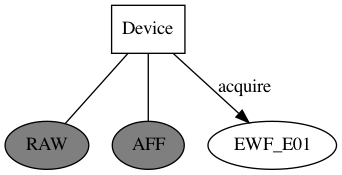
\includegraphics[width=.5\textwidth]{figures/device-to-image.png}
  \caption[Focus on EWF\_E01]{The default imaged format is EWF\_E01.}
  \label{fig:ewfe01}
\end{figure}

As shown in \cref{fig:ewfe01} the default file format for forensic images in the Lower Saxony Police is the Expert Witness Format (EWF\_E01). \cite{EWF}

Hellonium has to be able to process this file format.

\section{User interface}
\label{sec:gui}

In order to provide access to Hellonium for the less technically experienced investigators, it has to contain some kind of graphical user interface (GUI).

\section{Open Source}
\label{sec:oss}

Open source should be preferred. On the one hand, this allows Hellonium to be assembled according to the modular principle and, on the other hand, all functionalities can be checked using the source code.

\section{Metadata}
\label{sec:metadata}

The user has to be able to identify that the forensic image belongs to the case he is currently working on. To do this, Hellonium has to be able to extract the metadata embedded in shell of the EWF\_E01 container.

\section{Verification}
\label{sec:verification}

\subsection{EWF\_E01}

In order to ensure that the chain of custody is unbroken and the evidence integrity is untouched (digital forensic process), Hellonium must be able to calculate hash values over the contents of the EWF\_E01 container. The result has to be compared with the hash values stored in the metadata from the shell of the EWF\_E01 container. It has be pointed out if they do not match.

Following current, widely used forensic software, at least the hash variants MD5 and SHA1 must be supported.

\subsection{Digital signatures}

To prevent an unauthorised person from manipulating the evidence unnoticed and subsequently creating a new forensic image including new hash values, Hellonium has to be able to verify digital signatures. \cite{Nikkel2016:154}

Signify\footnote{https://www.openbsd.org/papers/bsdcan-signify.html}, minisign\footnote{https://jedisct1.github.io/minisign/}, GnuPG\footnote{https://www.gnupg.org/gph/en/manual/x215.html} and s/mime\footnote{https://tools.ietf.org/html/rfc8551} are widely used. At least one system has to be supported.

\subsection{RFC-3161 Timestamping}

In addition, to prevent also an authorised person from manipulating the evidence unnoticed afterwards and subsequently creating a new forensic image including new hash values, Hellonium has to be able to verify timestamps according to RFC-3161. \cite{Nikkel2016:154}

\section{Direct access storage device}
\label{sec:dasd}

A Direct access storage device (DASD) is one on which each physical record has a discrete location and a unique address. Thus records can be stored on a DASD in such a way that the location of any one record can be determined without extensive searching. Records can be accessed directly as well as serially. \cite{IBM1974}

In the case of the Master's thesis, this basically means hard disk drives and solid state disks.

\subsection{Partition scheme}

A partitioning scheme is a logical structure that are required for the operating system to access the storage space on the physical device. Logical structures include partition tables such as an master boot record (MBR) or GUID partition table (GPT). \cite{Aarnes2017:156}

Both partition schemes have to be interpretable.

\subsection{Partition Table}

During the creation of a partition, an ID (MBR) or a GUID (GPT) is specified, which is intended to save the information which file system will later be used in that partition, but does not necessarily have to.

\begin{figure}[htbp]  % order of priority: h here, t top, b bottom, p page
  \centering
  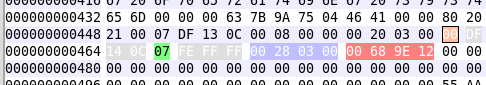
\includegraphics[width=.5\textwidth]{figures/wxhexeditor-mbr-ntfs.png}
  \caption[NTFS partition entry in MBR]{The screenshot shows a partition entry of a NTFS partition in a MBR.}
  \label{fig:NTFSMBR}
\end{figure}

The green marked ID (07) in \cref{fig:NTFSMBR} indicates that the partition is to be formatted with an NTFS file system.

Since the type of partitioning of the data carrier, based on the entries in the partition table, can already provide the first clues about operating systems that may be contained, Hellonium has to be able to correctly interpret the structure of data carriers with a Master Boot Record (MBR) as well as a Globally Unique Identifier Partition Table (GPT).

On Apple Macintosh devices with Bootcamp, a hybrid MBR can lead to confusion in this context. \cite{HybridMBR}

This circumstance must also be taken into account in Hellonium.

\subsection{Deleted partitions}

Hellonium has to be able to recognise if partitions have been set as new (empty) or non-existent (deleted) in the partition table in order to hide the relevant areas. Likewise, it has to be able to identify partitions that have only been quick formatted with another file system.

If such system volumes can be successfully restored, it should also be possible to boot from them again.

\section{Read only access}
\label{sec:readonly}

For information retrieval (preview/triage) only forensic tools should be used that require read access to the forensic image.

However, if partitions, file systems, RAID arrays or LVM2 volumes have to be recovered, write access has to be enabled in a forensic sound manner.

At the latest for emulating or virtualising an operating system contained in a forensic image, write access is required in the same way.

\section{Volumes}
\label{sec:volumes}

\subsection{File systems}

A file system stores data on a device so data can be retrieved by the system or a user. File systems are largely independent of an operating system (OS), and different file systems can be supported on different OSs when necessary drivers are installed. \cite{Aarnes2017:160}

It has to be possible to interpret as many file systems as possible.

\begin{figure}[htbp]  % order of priority: h here, t top, b bottom, p page
  \centering
  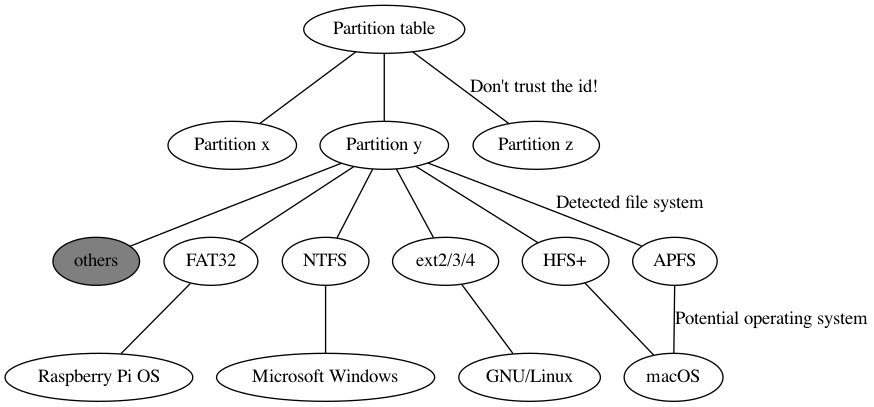
\includegraphics[width=.5\textwidth]{figures/fs-vs-os.png}
  \caption[File system and operating system]{The file system is one hint for the operating system.}
  \label{fig:fsandos}
\end{figure}

In addition to the partition table, it has to be possible to identify a file system in the partition itself, since both specifications do not necessarily have to match. An incorrect specification of the file system in the partition table can prevent Microsoft Windows from starting. GNU/Linux, BSD and Unix are not affected by this restriction. On the basis of the actual file system, one can narrow down or even determine the containing operating system analogous to the partition table. The tool used must therefore be able to recognise not only mainstream, i.e. FAT32 and NTFS, but also HFS+, APFS and ext2/3/4. Support for even more file systems is welcome.

\subsection{Root directory}

The folders contained in the root-directory can strengthen or weaken initial assumptions about the contained operating system.

\subsection{Certain files}

The simple presence of certain files can also strengthen or weaken initial assumptions about the operating system they contain. In addition to a direct interpretation of the contents, it must also be possible to extract them for further external processing.
In order to ensure the chain of custody and evidence integrity (digital forensic process) even after extraction, it must be possible to easily create hash values for the extracted data.
The content of certain files can even substantiate the assumptions regarding the version/release.
For this purpose, the tool used must not only be able to interpret the Windows Registry (mainstream). It must also be able to interpret plist (macOS) and simple text files (GNU/Linux).

\section{Files}
\label{sec:files}

For later successful virtualisation, not only the version of the operating system is interesting. An older version may require a different recipe than a current version. 
However, not everything is needed that is often used for preview or triage. 

\section{Password}
\label{sec:password}

Every secured computer system must require all users to be authenticated at login time. After all, if the operating system cannot be sure who the user is, it cannot know which files and other resources he can access. Password protection is based on something the user knows. The simplest implementation just keeps a central list of logins and passwords. The login typed in is looked up in the list. If they match, the login is allowed. \cite{Tanenbaum2014:626}

In modern operating systems, passwords are not stored in plain text. They are converted to so-called hash values using mathematical one-way functions before they are stored.

Hellonium should offer several ways to find or calculate passwords from hints or hash values.

\subsection{Microsoft Windows}

In addition to the Windows version, the time zone, password information and network configuration can be read from the Windows registry.
When reading out the password hash values, it must be ensured that both the old (before Windows 10 Anniversary Update) and the new (as of Windows 10 Anniversary Update) procedure for storing the hash values in a hidden manner is supported.

\subsection{Apple macOS}

The information about the operating system version, the time zone, the password instructions and the password hashes are stored under macOS in so-called plists (plain text or binary XML files). Hellonium has to be able to interpret both versions.

At least the last three forms (up to 10.6, 10.7 and from 10.8) of password hashes hast to be correctly extracted from the plists.

If autologin is enabled, the password of the user who is automatically logged in is obfuscated and stored in the file /private/etc/kcpassword. Hellonium has to be able to defuscate the password.

\subsection{GNU/Linux}

Under GNU/Linux it often happens that after successful virtualisation you find yourself on the command line and not on a graphical desktop.
In this case it is good to know which operating system you are dealing with and which steps have to be taken so that the graphic desktop can be reactivated afterwards.

The information about the operating system version and the password hashes can be directly taken from plain text files.

The information about the time zone has to be obtained via the copy or a symbolic link to a corresponding zone file in /usr/share/zoneinfo. Hellonium has to be able to correctly determine the time zone.

\subsection{Raspberry Pi}

In addition, in the case of a Raspberry Pi, it is important to be able to find out the CPU and kernel version, as an appropriately prepared kernel has to be "injected" from the outside. 

If the kernel is incompatible with the original kernel, it may not be possible to load kernel modules afterwards.

Hellonium should already hold a selected choice of kernel versions for this purpose.

\section{Write access}
\label{sec:writeaccess}

Write access in a forensically sound manner is required as soon as changes to a corrupted partition table or file system are necessary.

Likewise, if login passwords need to be cleared.

In the case of an older version of Windows (XP, Vista or 7), the registry have to be changed in order to prevent the Blue Screen of Death (BSOD) immediately after start-up.

Under macOS, a new account with administrator rights can be created by just deleting the file /private/var/db/.AppleSetupDone.

\section{Virtualization}
\label{sec:virtualization}

Depending on the operating system and/or operating system version, the correct choice of virtual hardware also influences whether the system can be booted successfully or not.

It must at least be possible to boot Microsoft Windows, Apple MacOS and GNU/Linux incl. Rapberry Pi OS.

\subsection{Firmware}

\begin{figure}[htbp]  % order of priority: h here, t top, b bottom, p page
  \centering
  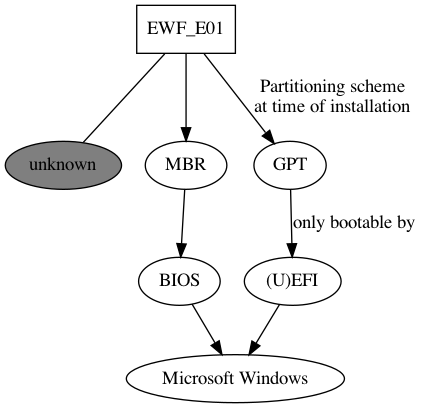
\includegraphics[width=.5\textwidth]{figures/ps-vs-firmware-win.png}
  \caption[Windows fireware dependency]{Micosoft Windows doesn'l like firmware switching.}
  \label{fig:firmware}
\end{figure}

Because Microsoft Windows can only be booted with a BIOS if it was installed with it and can only be booted with a UEFI if it was installed with it, it has to be possible to boot a guest OS with both a BIOS and a UEFI.

\subsection{Network card}

For older operating systems, it should be possible to provide an older network card that is as widely used as possible, as no drivers may have been installed for newer ones.
For newer operating systems, it should be possible to provide a new, current network card that is as widespread as possible, as drivers for older ones may no longer be available for current operating systems.

To prevent unnecessary restarts, the network card should always be available from the beginning.

However, to prevent e.g. remote wiping or the spread of potentially existing malware, the virtual network cable should not be connected by default. A connection should be possible after checking during operation.

\subsection{CPU}

In particular, older 32-bit versions of Windows, which were installed on hardware with only one processor core, occasionally fail to start on a 64-bit system with several cores.

It has to be possible to adjust the CPU in relation to 32- or 64-bit, cores and threads.

\subsection{Apple SMC}

Without this chip, virtualisation of Apple macOS is not possible.

So it has to be possible to offer the chip virtually with correct data.

\subsection{ARM}

A full virtualisation of ARM is unfortunately not possible on Intel/AMD because they are not binary compatible.

Since the Raspberry Pi with ARM SoC has become very popular and is increasingly used as a home server, it has to be possible to emulate an ARM SoC.

\subsection{NVMe}

In some GNU/Linux installations it happens that in /etc/fstab disks are still addressed with device names and not with a label or a UUID. If NVMe is used the name of the device differs from the other ones.

To enable virtualisation without additional changes in the file system, at least IDE, SATA, SCSI, SAS and NVMe controllers should be offered.

\section{Drivers}
\label{sec:drivers}

To enable a display without unnecessary delays and to be able to adjust the resolution beyond VGA resolution, appropriate drivers should be offered for the virtual graphics cards if possible.

\section{Export}
\label{sec:export}

In principle, Hellonium should be user-friendly that remote access or export of the virtual machine should no longer be necessary.

It can still be offered.
